\subsection{Introducción}

Go.JS \cite{gojs} es una biblioteca de JavaScript para implementar editores gráficos dentro de interfaces web. GoJS facilita la implementación de funciones tales como definición de símbolos gráficos, gestión de paletas de símbolos, arrastrar y soltar (\emph{drag and drop}), copiar y pegar, edición de etiquetas de texto asociadas a símbolos gráficos, menús contextuales, función de deshacer o gestión de eventos, entre muchas otras funcionalidades.

Para ilustrar el funcionamiento de GoJS, a continuación se muestra un ejemplo sencillo de creación de editor gráfico de grafos
para el dibujo de círculos interconectados por flechas. Dicho editor se muestra en la Figura\ref{fig:gojssample}.

%%=================================================================================================%%
%% NOTA: Todas las imágenes con sus números de líneas y sintaxis coloreada si puede ser            %%
%%       Hay una librearía en Latex (listing) se llama                                             %%
%%       Puedes copiar y pegar de aquí y te vale para Javascript https://goo.gl/6CstHr             %%
%%=================================================================================================%%

\begin{figure}[!tb]
	\centering
	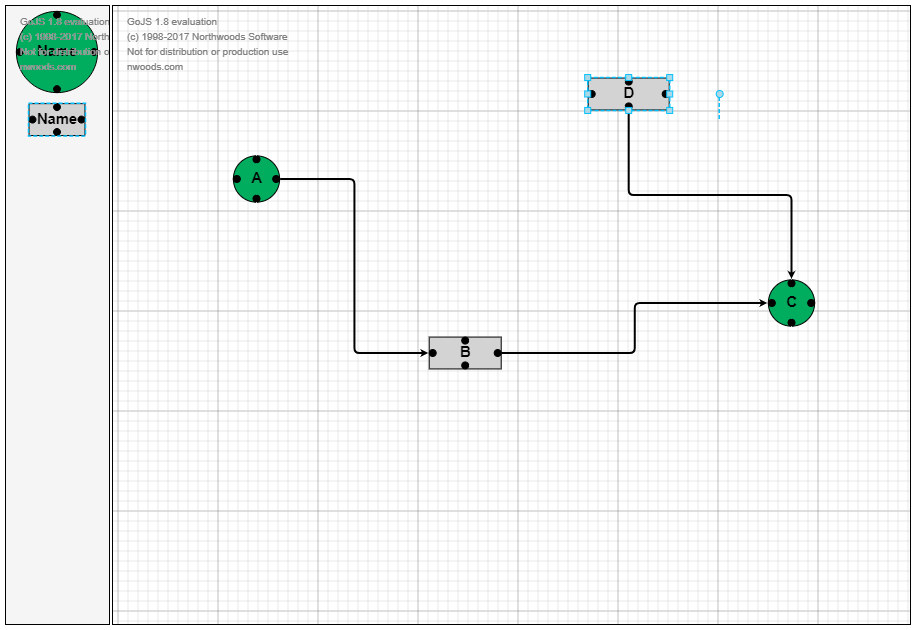
\includegraphics[scale=0.75]{gojssample.png}
	\caption{Editor gráfico creado en GoJS}
    \label{fig:gojssample}
\end{figure}

Para empezar, cabe destacar que, para poder crear este editor, es necesario reservar dos secciones de la página HTML que lo contiene. Una sección para la paleta contenedora de los elementos gráficos del editor, que en este caso es sólo el círculo, y otra sección para el diagrama sobre el que se depositarán los elementos gráficos. 

\begin{figure}[!tb]
	\centering
	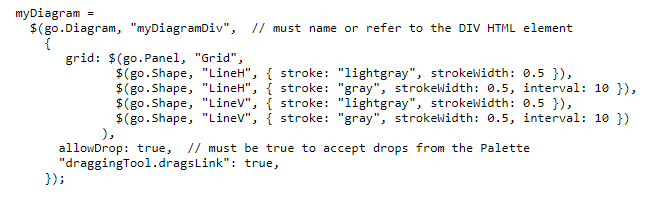
\includegraphics[scale=0.90]{creacionDiagramaGoJS.png}
	\caption{Especificación del área de dibujo.}
    \label{fig:creacionDiagramaGoJS}
\end{figure}

A continuación, deben realizar una serie de acciones a nivel de Javascript para proporcionar tanto a la paleta de dibujo como al área de dibujo del comportamiento deseado. En primer lugar, crearemos una variable \texttt{\$} que dé acceso al entorno GoJS. Esto se realiza mediante la llamada a la sentencia \texttt{make} de librería \emph{GraphObject} de GoJS (Figura \ref{}, Líneas XX-YY).

Seguidamente, se personaliza la sección HTML reservada al diagrama, denominada \texttt{myDiagramDiv} (Figura \ref{}, Líneas XX-YY), asignándole un \emph{\emph{grid}} o cuadrícula de fondo (Figura \ref{}, Línea XX), especificando los colores de las líneas de la cuadrícula (Figura \ref{}, Líneas XX-YY) y dándole la capacidad de poder arrastrar elementos sobre él (Figura \ref{}, Líneas XX).

%%========================================================================%%
%% NOTE(Pablo): Hasta aquí va más o menos bien la cosa, pero aquí         %%
%%    empezamos a perder el hilo. ¿De dónde han salido los círculos y     %%
%%    qué es un puerto. Lo normal es explicar primero cómo se añaden      %%
%%    círculos a la paleta, qué es un puerto, la necesidad de crearlos,   %%
%%    y luego ya cómo se crean.                                            %% 
%%========================================================================%%

\begin{figure}[!tb]
	\centering
	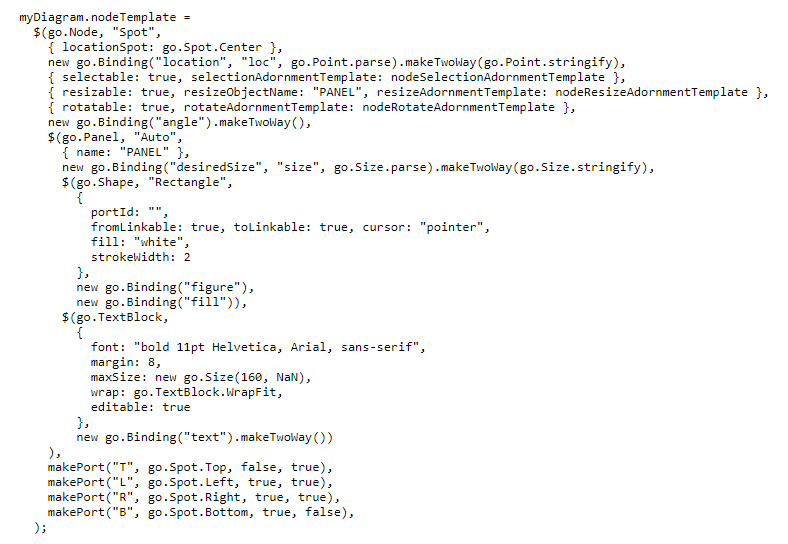
\includegraphics[scale=0.90]{nodeTemplate.png}
	\caption{Especificación de los círculos como nodos.}
    \label{fig:nodeTemplate}
\end{figure}

La Figura \ref{} muestra cómo se crean los \emph{nodos} de un diagrama. Los nodos son todos aquellos elementos de los que se va a componer el diagrama. En nuestro ejemplo, estos nodos son los círculos. Para crear la definición un nodo lo primero es declarar el nodo con \texttt{\$(go.Node} (Figura \ref{}, Líneas XX). A continuación, especificamos, mediante la definición de ciertas propiedades, cómo se comportará el nodo (Figura \ref{}, Líneas XX). En nuestro caso, se indica que %% esto del template no lo entiendo muy bien. (Figura \ref{}, Líneas XX),
y que el nodo, dentro del área de dibujo, podrá ser seleccionado, redimensionado y rotado (Figura \ref{}, Líneas XX, YY y ZZ, respectivamente).

%% el ejemplo se le da una localización en el template\footnote{El template es el espacio que alberga, y sobre el que se definen
%% las estructuras que definen un nodo.}

%%=========================================================================%%
%% NOTE(Pablo): Si los nodos van a tener nombre, que se vea también en el  %%
%%    ejemplo. ¿Ésto es necesario ponerlo siempre en Go o se puede omitir? %%
%%=========================================================================%%

Cada nodo poseerá además una etiqueta de texto que permitirá especificar su nombre, denominada \emph{panel} (Figura \ref{}, Líneas XX-YY). En nuestro caso, dicho panel poseerá una forma rectangular (Figura \ref{}, Líneas XX) y una fuente con unas características determinadas. 

Una vez definidas las propiedades básicas de un nodo, el siguiente paso es definir cómo enlazar dichos nodos. Para ello debemos definir dos elementos: \emph{puertos} y \emph{enlaces}. Los puertos de un nodo son los puntos de un nodo desde los cuáles dicho nodo se puede enlazar con otros nodos. Para añadir puertos a los círculos creamos una función determinada, la cual se muestra en la Figura \ref{}. %% Describir algo del código que aparece. 
A continuación, añadimos cuatro llamadas a esta función a la declaración de los círculos como nodos, con el objeto de crear un puerto a cada lado del eje de un círculo (Figura \ref{}).

%%=========================================================================%%
%% NOTE(Pablo): La figura donde se añaden los cuatro makePort hay que      %%
%%   hacerla nueva                                                         %%
%%=========================================================================%%

%%=========================================================================%%
%% NOTE(Pablo): ¿Por qué los parámetros tres y cuatro cambiando de true    %%
%%   a false a veces?                                                      %%
%%=========================================================================%%

\begin{figure}[!tb]
	\centering
	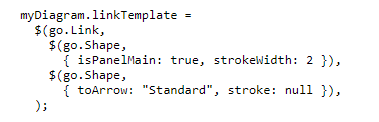
\includegraphics[scale=0.90]{linkTemplate.png}
	\caption{Especificación del comportamiento entre círculos.}
    \label{fig:linkTemplate}
\end{figure}

Una vez definidos los puertos, especificamos cómo se comportarán los enlaces entre nodos, tal como muestra la Figura \ref{}. %% Comentar un poco más aquí sobre el código.

\begin{figure}[1tb]
	\centering
	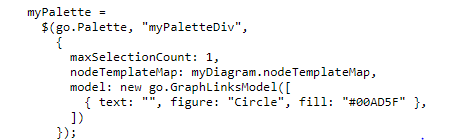
\includegraphics[scale=0.90]{palette.png}
	\caption{Paleta de Nodos}
    \label{fig:palette}
\end{figure}
\vspace{5mm}

Por último, creamos la paleta de herramienta, tal como se muestra en la Figura \ref{}. Como se puede observar, la paleta se sitúa sobre una sección HTML denominada \emph{myPalleteDiv}. 

%% A dicha paleta asocia  los nodos y se le añade al modelo de datos de la paleta un elemento círculo de color verde y sin texto en su interior.

Una vez definidos estos elementos, nuestro editor gráfico queda implementado ya que GoJS se encargará de dibujar los elementos sobre el área de dibujo cuando estos son seleccionados en la paleta, permitiendo arrastrarlos, redimensionarlos o renombrarlos, entre otras funciones. Por tanto, GoJS nos permite obtener fácilmente editores gráficos en Javascript a partir de la especificación
de las propiedades que compondrán dicho editor. Concretamente, el editor de la Figura \ref{} se puede implementar con sólo XX líneas Javascript.     